
\subsection{实验先问什么：不增加电流方向，材料这一步还能更好吗？}
前面的机制推导告诉我们，一个方向对材料有无作用，要经过材料进入、内部反馈和接收返回。接下来要把这个认识变成可以检验的设计：已经用接收谱选好一个电流空间，能否只换掉一两个方向，就使它生成的材料步更接近完整模型？

这里采用接收基底（receiver backbone）作为起点。它是接收算子中最容易辐射到测量端的方向组合。完整参考保持不变；当前材料、总场、六次照明、残差和正则项也保持不变。交换（exchange）只改变线性化内部使用的电流子空间。因此，改善不是增加了数据，也不是更换了材料先验。

四类对象为平滑介质、近接触结构、分层结构和非对称多物体；前两类使用Gaussian材料切向，后两类使用voxel材料切向。每个对象取初始、中期和晚期三个已保存状态，分别保留4、8、16列共享复电流。共36个状态--预算单元，实际是四个物理对象，不是36个独立物体。

为区别“存在好方向”和“能便宜地找到它”，实验设置三个层次。局部参考搜索（local teacher）在声明的完整交换字典中计算真实完整收益；代理搜索（surrogate search）按更丰富但仍约化的模型排序；定向复核（directed verification）只对每轮最多两个finalist计算完整$Jd$，接受真实收益超过数值阈值的动作。每条路径最多接受三个动作。接受以后重新计算条件因素，不把第一轮得分沿用到底。

\subsection{怎样衡量材料步：完整GN差距不是图像误差}
完整二次目标$\Phi$有唯一最优步$s_*$。约化电流模型产生$s_U$，比较
\[
R_{\rm GN}(U)=\Phi(s_U)-\Phi(s_*)
=\tfrac12(s_U-s_*)^TH(s_U-s_*).
\]
它是完整Gauss--Newton二次差距（full-GN quadratic gap），表示“这一步和完整模型应给的步差多少”。它没有量化最终图像是否恢复了真实边界。正收益$Q$意味着$R_{\rm GN}$下降，负收益意味着它上升。

风险比（risk ratio）以同一个对象、同一批状态和预算的receiver为分母。先求和再相除，避免某个极小分母单元主导结论：
\[
\rho_{\rm object}=
\frac{\sum_{\mathrm{state},k}R_{\rm verified}}
{\sum_{\mathrm{state},k}R_{\rm receiver}}.
\]
比值0.2表示这一对象汇总的完整GN差距剩20\%，并不是材料重建误差只有20\%。

\begin{center}\small
\begin{tabular}{@{}lrrr@{}}\toprule
对象 / 材料表示&Local teacher风险比&Verified风险比&两路径收益取得比例\\\midrule
平滑 / Gaussian&0.0984&0.1904&89.8\%\\
近接触 / Gaussian&0.2016&0.6538&43.4\%\\
分层 / voxel&0.1520&0.2776&85.2\%\\
非对称 / voxel&0.1628&0.4181&69.5\%\\\bottomrule
\end{tabular}\end{center}
四对象的verified风险比中位数为0.34785，相当于差距降低约65.2\%。35个单元有可分辨改善，一个单元保持不变，36个单元没有可分辨退化。这是固定电流维数上的正面设计结果。Teacher的结果仍是声明邻域和最多三个动作中的局部参考，不是所有电流空间的全局最优。

\begin{figure}[htbp]\centering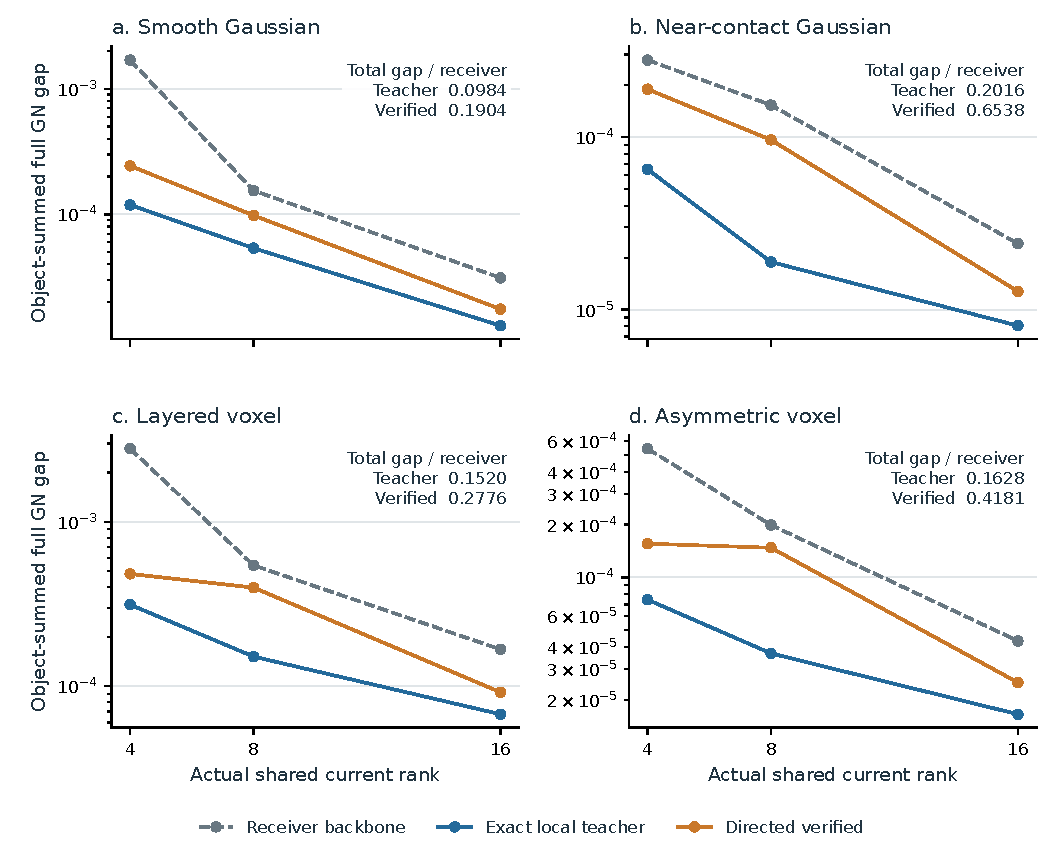
\includegraphics[width=\linewidth]{figures/exchange_risk.pdf}
\caption{完整GN差距按对象和电流维数汇总。灰线为receiver不动，蓝线为声明域的local teacher，橙线为受限候选加定向复核。纵轴为对数，三个状态在各点求和。蓝线与橙线的差包含候选覆盖及多步路径差，不能统称为纯评分误差。}
\end{figure}

\subsection{发现瓶颈：评分已经准确，短候选池仍会漏掉机会}
可以在共同receiver起点上，只比较一次决定，避免不同路径互相混淆。设各checkpoint的最好非负收益是$Q_{\max,c}$。对每个对象的九个共同起点，先把anchor所挑动作的真实gain求和，再除以$\sum_c Q_{\max,c}$，对象级捕获率为98.1--99.6\%。这是gain加权汇总，不是每个checkpoint的下界；少数checkpoint的anchor top-one仍会选到负gain，部署复核会拒绝它。这个汇总说明完整字典内的代理模型已经辨认很大部分机会。

在线程序只允许十二个incoming候选，以控制费用。这个短候选池（shortpool）本身包含的最好收益，在平滑、近接触、分层和非对称对象上，分别是完整邻域的96.9\%、35.3\%、92.0\%和65.9\%。近接触对象即使把短池内所有得分都算准，也拿不到池外的好方向。这比单纯观察“代理方法没有达到teacher”更有解释力：应该优先改善候选从哪里来，而不是假定必须换一个更复杂的评分器。

这里的机会捕获率（opportunity capture）针对同一checkpoint、同一动作语义，不能与表中多步路径的收益比例混用。复杂几何上的candidate coverage与条件耦合，是目前最直接的算法设计问题。

\subsection{信息诊断回答另一个问题：模型声称能辨认多少材料方向}
固定物理材料坐标后，数据曲率是$\mathsf I_U=J_U^TJ_U$。选定正定尺度$P=10^{-5}I$，由
\[
P^{-1/2}\mathsf I_UP^{-1/2}w_i=\nu_iw_i
\]
得到尺度归一化的材料响应。信息体积（information volume）和有效维数（effective dimension）定义为
\[
\mathcal D(U)=\tfrac12\sum_i\log(1+\nu_i),
\qquad d_{\rm eff}(U)=\sum_i\frac{\nu_i}{1+\nu_i}.
\]
第一个量表示局部响应谱的体积尺度；第二个量平滑衡量相对于$P$有作用的方向数。这里的measurement normalization没有实测噪声协方差认证，因此不把它们直接称作已校准的互信息。

还要区分信息幅度（information magnitude）与信息保真度（information fidelity）：前者问约化模型声称有多少响应，后者问该曲率离完整模型有多远。更大的曲率可能只是模型放大了敏感度；而更接近完整曲率，也没有单独确定当前步，因为$J^Tr$同时参与了正规方程。

一个真实近接触对象的rank4交换，同时得到：
\[
\Delta\mathcal D=+6.3127,\qquad
\Delta d_{\rm eff}=+1.8613,\qquad
Q_{\rm full}=-5.5754\times10^{-5}.
\]
它的信息体积更大、有效维数更高，某个归一化曲率fidelity还略有改善，却使完整材料步更差。这不是一个抽象$2\times2$例子，而是保存了状态、基底、步和方向场的vector-Maxwell交换。公式
\[
d=-H_n^{-1}(\Delta h+\Delta\mathsf I\,s_o)
\]
指出必须共同考虑的两部分：谱所描述的曲率改变，以及与residual相连的$\Delta h$。该见证没有孤立证明其中哪一项主导。一个强响应若与当前需要修正的残差方向不匹配，不会自动变成好更新。

Gaussian中计算的是完整54维实材料空间；voxel中信息诊断仅在相同的十六维材料探针空间计算，不能把其谱当作整个3456维材料空间的谱。

\begin{figure}[htbp]\centering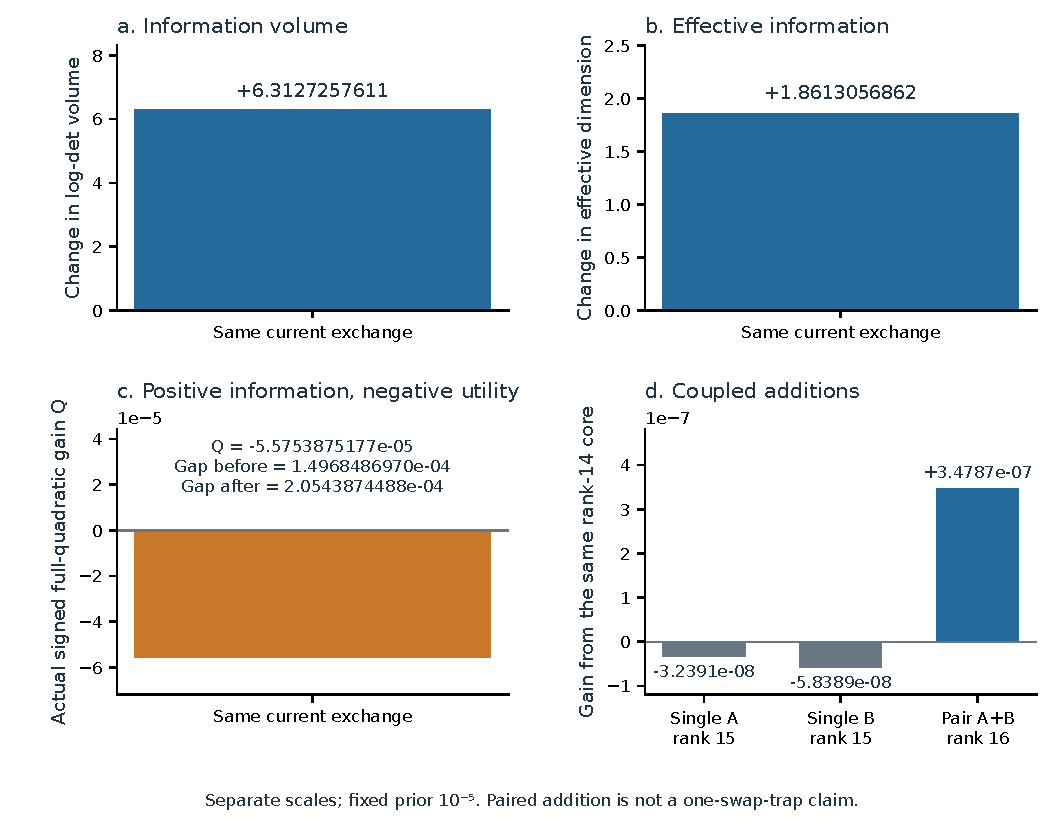
\includegraphics[width=\linewidth]{figures/information_and_pair_witness.pdf}
\caption{同一Maxwell替换的信息体积、有效维数和实际收益使用各自量纲。右下图另展示共同rank14核心上的两个单列添加与联合添加；它们不是同秩交换，也不证明所有贪心方法必然失败。}
\end{figure}

\subsection{为什么要重算条件得分：两个不好的单独动作可能组成好动作}
从同一个rank14核心开始，分别加入两个方向，完整收益为
\[
Q_A=-3.2391\times10^{-8},\qquad
Q_B=-5.8389\times10^{-8}.
\]
单看任一个都不值得加。但一起加到rank16，收益变成
\[
Q_{A+B}=+3.4787\times10^{-7}.
\]
这个配对相互作用（pair interaction）来自同一物理核心和共同目标下的计算。540个预先固定pair测试中，有5个严格满足“两单列非正、联合为正”。数量只描述该测试集合，不能当作所有电流中这种现象的概率。它提示我们：在singleton判断不明确时，小规模block proposal可能比独立按单列分数排序更有价值。

另一个受控实验把两个因素拆开。$v$是旧曲率给出的线性化位移，$d$是新旧模型实际最优步差；同一批候选分别用线性或完整二次表达式评分，最后统一执行真实$d$。强制选择top-one、不含no-op时，对真实$d$只看线性项，会在29/36个单元挑到负收益；保留二次项后降到1/36。这个计数说明该共同候选诊断中的有限位移惩罚不可省略。实际部署另有no-op和完整gain复核，拒绝负收益动作。

旧大样本finite/first-order风险比0.1171同时改变了方向构造和terminal swap，不能单独归因于曲率项。这里的共同候选诊断才真正把两个因素分开。

\subsection{计算费用：使用完整物理方向，仍能把复核限定在少量动作}
验证不要求先构造full Jacobian。当前输出$Jx$可缓存；某个动作产生$d$后，只计算$Jd$，代入定向收益公式。六次illumination意味着单个方向需要六份current RHS。75个接受动作共支付1164份finalist tangent RHS，另有初始化、候选投影、teacher和离线评价费用。

相同CUDA FP64物理算子的五次轮换计时中，近接触Gaussian三个预算的conditional warm selection为0.594、1.418、2.690秒；分层voxel为0.891、1.153、3.400秒。只做一次同池决定更便宜；固定one-pass surrogate也更便宜，但检查的信息和接受语义不同。这里的价值是付出可见费用换取完整步保真度，尚未测得比receiver不动更快的冷启动反演。

全部远端作业占用为4889.515秒，即81.49分钟，包含17次作业、两次失败、teacher、诊断和付费预热。显存峰值1872MiB，没有OOM。这个作业占用不是GPU始终繁忙的时间，也不是某一个selector的单次费用。

\subsection{学习、停止与重建分别回答什么}
对象分组的小网络只预测候选优先级：两对象训练，一对象validation，一对象test。三个seed的MLP在heldout对象取得teacher top-two收益的98.85--99.16\%，但现有anchor规则达到99.885\%；group-mean模型为75.99--98.03\%。网络没有带来超越解析规则的收益，也没有完成新物理验收和全费用减半，因此不承担论文算法创新。

高精度方向检查没有给出严格的output-error bound。22个单元为未解决停止（abstention），14个达到动作上限；它们都不称全邻域局部最优。允许$\le k$的策略最终仍全部用满$k$，没有取得终态节省电流秩。

最后，一次无约束$\alpha=1$材料步相对初始材料，在19个单元更接近真值，17个更远，28步违反材料约束。该诊断没有经过line search，既不是与receiver最终材料端点的比较，也不是nonlinear reconstruction结果。论文的明确正面结果是同预算的完整GN更新改善；约束接受、噪声及最终图像恢复，构成下一层证据问题。
